\chapter{ម៉ាសុីន}
\section{លំនាំអាដ្យាបាទិច}
\begin{definition}
	លំនាំអាដ្យាបាទិច ជាលំនាំដែលថាមពលកម្តៅមិនប្តូរជាមួយមជ្ឈដ្ឋានក្រៅ(មិនស្រូប និងមិនបញ្ចេញកម្តៅ) ឬមានតម្លៃថេរជានិច្ច $\left(\Delta Q=0\right)$។ តាមច្បាប់ទីមួយទែម៉ូឌីណាមិចយើងបានៈ $W=-\Delta U$។
\end{definition}
\begin{example}
	\begin{enumerate}[m]
		\item កាលណាឧស្ម័នត្រូវបានបណ្ណែនតាមបែបអាដ្យាបាទិច កម្មន្តបានធ្វើទៅលើឧស្ម័ននោះគឺ $640J$។\\ គណនាបម្រែបម្រួលថាមពលក្នុងរបស់ឧស្ម័ន។
		\item ក្នុងប្រព័ន្ធត្រមោចមួយ បើថាមពលក្នុងថយចុះ $500J$ តើកម្មន្តដែលបំពេញដោយប្រព័ន្ធនោះស្មើនឹងប៉ុន្មាន?
	\end{enumerate}
\end{example}
\section{ម៉ាសុីនទ្រឹស្តី(ម៉ាសុីនកាណូ, ម៉ាសុីនអុីដេអាល់)}
\subsection{ម៉ាសុីនកម្តៅ}
\begin{definition}
	\emph{\kml ម៉ាសុីនកម្តៅ{\en(Heat Engine)}} ជាឧបករណ៍ ឬម៉ូទ័រទាំងឡាយណាដែលបម្លែងថាមពលកម្តៅទៅជាកម្មន្ត។\\ ដែលគេអាចហៅយ៉ាងខ្លីថា "ម៉ាសុីន" មានម៉ាសុីនម៉ូតូ ម៉ាសុីនឡាន ម៉ាសុីនភ្លើង។ល។
\end{definition}
\begin{minipage}[l]{.5\textwidth}
	ឧទាហរណ៍គំរូនៃប្រភេទឧបករណ៍នេះ គឺម៉ាសុីនចំហាយទឹកដែលអាចសង្ខេបយ៉ាងងាយបានដូចរូបខាងក្រោម។
	ដំណើរការរបស់វាគឺដំបូងគេប្រើប្រាស់ឥតន្ធនៈដើម្បីបង្ហូរទឹកក្នុងឆ្នាំងដាំទឹក(ប្រភពធុងក្តៅ) ដែលបង្កើតឲ្យមានចំហាយ រួចហើយឲ្យចំហាយនោះចូលក្នុងម៉ាសុីនឡើងវិញដែលនៅពេលនោះវារីកមឌដោយអាចធាក់ពីស្តុងដើម្បីធ្វើកម្មន្ត(មើលរូប)។
\end{minipage}
\begin{minipage}[r]{.6\textwidth}
	\begin{figure}[H]
		\centering
		\begin{tikzpicture}
			\node at (0,0) {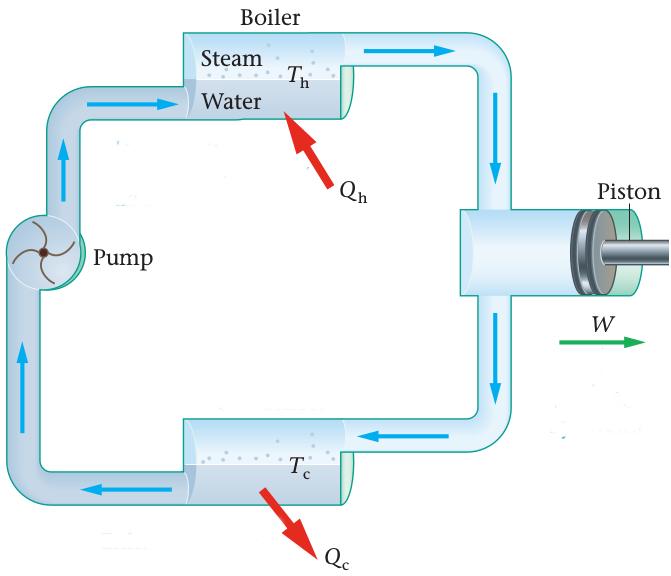
\includegraphics[scale=.3]{heat-engine}};
			\node at (-1.7,.2) {\fontsize{10}{10}{\text{\DS ម៉ាស៊ីនបូម}}};
			\node at (-.5,-1) {\fontsize{10}{10}{\text{\DS ករជាញើស}}};
			\node at (-.5,3.1) {\fontsize{10}{10}{\text{\DS ឆ្នាំងដាំទឹក}}};
			\node at (3.5,1.2) {\fontsize{10}{10}{\text{\DS ពីស្តុង}}};
			\node at (.3,1) {$Q_{h}$};
			\node at (.1,-2.8) {$Q_{c}$};
			\node at (3.2,-.5) {$W$};
			\draw (3.1,.5) -- (3.1,1.2);
			\draw[->, line width=2pt] (2.7,-.8) -- (3.7,-.8);
		\end{tikzpicture}
		\caption{ម៉ាសុីនចំហាយទឹក}
	\end{figure}
\end{minipage}
នៅពេលដែលពីស្តុងផ្លាស់ទីវាអាចធ្វើឲ្យកង់ស្ពឺនៃយានអាចវិលបាន(គឺបំពេញកម្មន្តទៅមជ្ឈដ្ឋានក្រៅបាន)។ បន្ទាប់ពីចាកចេញពីម៉ាសុីន ចំហាយមួយចំនួន ក៏បន្តទៅតំបន់ដែលចំហាយឲ្យករទៅជាទឹក(ប្រភពធុងត្រជាក់)។\\
គ្រប់ម៉ាសុីនកម្តៅទាំងអស់ស្រូបកម្តៅពីប្រភពដែលមានសីតុណ្ហភាពខ្ពស់ ដើម្បីបម្លែងជាកម្មន្តមេកានិច ហើយបញ្ចេញ ឬបំភាយកម្តៅខ្លះត្រង់ប្រភពត្រជាក់ ដែលដំណើការនេះត្រូវបានធ្វើដដែលៗ ជាវដ្តនៃដំណើការ{\en(Cycle)} ដែលបង្កើតបានជាបម្លែងបិទ។ តាមច្បាប់ទីមួយទែម៉ូឌីណាមិចៈ
\begin{flalign*}
	\Delta U = U_{2}-U_{1}=0\quad &\quad \text{ដូចនេះ}\quad W=Q\\
	\text{ដែល}\quad Q\quad \text{ជាបរិមាណកម្តៅសរុបនៃដំណើរការរបស់ម៉ាសុីន}\quad &\quad W\quad\text{ជាកម្មន្តសរុបដែលធ្វើដោយម៉ាសុីន}
\end{flalign*}
\begin{itemize}
	\item \emph{\DS ដ្យាក្រាម លំហូរនៃថាមពល}\\
	អ្វីដែលម៉ាសុីនប្រើកម្តៅទាំងអស់មានចំណុចដូចគ្នាមានដូចជាៈ
	\begin{enumerate}[m]
		\item ប្រភពដែលមានសីតុណ្ហភាពខ្ពស់ផ្តល់កម្តៅមួយផ្នែកសម្រាប់ធ្វើកម្មន្ត(កម្មន្តមេកានិច)។
		\item ប្រភពដែលមានសីតុណ្ហភាពទាបគឺមានតួនាទីសម្រាប់យកចំហាយទឹកដែលសល់ក្រោយពីកម្តៅធ្វើជាកម្មន្ត\\(កម្មន្តមេកានិច) ទៅជាទឹកឡើងវិញ។
		\item ដំណើរការរបស់ម៉ាសុីនគឺធ្វើឡើងក្នុងបម្លែងបិទ។
	\end{enumerate}
	\begin{minipage}[l]{.4\textwidth}
		\begin{flalign*}
			\text{គេមាន}\quad:&\quad W=Q\\ 
			\text{ដែល}\quad:&\quad Q=Q_{h}-Q_{c}\\
			\text{នោះ}\quad:&\quad W=Q_{h}-Q_{c} \\
			\text{ដូចនេះ}\quad:&\quad W=Q_{h}-Q_{c}\quad
		\end{flalign*}
	\end{minipage}
	\begin{minipage}[r]{.7\textwidth}
		\begin{figure}[H]
			\centering
			\begin{tikzpicture}[>={Triangle[angle=60:1 2]}, scale=1.5]
			\path [shading=heat]
			(-2,2) rectangle (2,3/2) (-2,-2) rectangle (2,-3/2);
			\draw (-2,3/2) -- (2,3/2) (-2,-3/2) -- (2,-3/2);
			\scoped{
				\clip (-3/2,-7/4) rectangle (3/2,7/4);
				\draw [shading=heat] 
				(3/4,2) -- (-3/4,2) -- (-3/4,7/4) arc (90:0:1/4) -- (-1/2,-3/2)
				arc (360:270:1/4) -- (-3/4,-2) -- (1/4,-2) -- (1/4,-7/4) 
				arc (270:180:1/4) -- (0,-3/2)    -- (0,1/4)   
				arc (180:270:1/2) -- (2,-1/4)  -- (2,1/4) -- (3/4,1/4)
				arc (270:180:1/4) -- (1/2,3/2)  arc (180:90:1/4) -- (3/4,2);
			}
			\path (0,2.6) node {\text{\DS ធុងក្តៅ} $T_h$} (0,-2.5) node {\text{\DS ធុងត្រជាក់} $T_c$} (0,2) node {$Q_{h}$} (-.2,-1.8) node {$Q_{c}$} (3.5,0) node {$W=Q_{h}-Q_{c}$} (2.7,1) node {\text{\DS ម៉ាសុីន}};
			\draw [red!75,  line width=1cm/4, ->] (0,3/2) -- (0,1/2);
			\draw [red!75,  line width=1cm/8, ->] (-1/4,-1/2) -- (-1/4,-3/2);
			\draw [blue!75, line width=1cm/8, ->] (1,0) -- (2,0);
			\draw (0,.2) circle (.8cm);
			\draw[->, line width=2pt] (2,1) -- (.7,.8);
			\end{tikzpicture}
			\caption{ដ្យាក្រាមតាងការបម្លែងថាមពលកម្តៅ}
		\end{figure}
	\end{minipage}
	\item \emph{\DS ប្រសិទ្ធភាពនៃម៉ាសុីនកម្តៅ(\en Efficiency)}
	\begin{flalign*}
		\text{គេមាន}\quad :&\quad W=Q_{h}-Q_{c}\\
		\text{គេបាន}\quad :&\quad e=\frac{W}{Q_{h}}=\frac{Q_{h}-Q_{c}}{Q_{h}}\\
		\text{ដូចនេះ}\quad :&\quad e=1-\frac{Q_{c}}{Q_{h}}
	\end{flalign*}
\end{itemize}
\begin{example}
	\begin{enumerate}[m]
		\item ម៉ាសុីនកម្តៅមួយស្រូបកម្តៅ $200J$ ពីធុងក្តៅដើម្បីធ្វើកម្មន្ត និងបំភាយកម្តៅអស់ $160J$ ទៅធុងត្រជាក់។ គណនាទិន្នផលកម្តៅនៃម៉ាសុីន។
		\item ម៉ាសុីនកម្តៅមួយធ្វើកម្មន្ត $9200J$ ក្នុងមួយវដ្ត ខណៈដែលវាស្រូបកម្តៅ $25.0kcal$ ពីធុងដែលមានសីតុណ្ហភាពខ្ពស់។ គណនាទិន្នផលនៃម៉ាសុីនកម្តៅនេះ។
		\item ម៉ាសុីនមួយបញ្ចេញកម្តៅ $8200J$ ខណៈពេលដែលម៉ាសុីនធ្វើកម្មន្តបាន $2600J$។\\ គណនាទិន្នផលនៃម៉ាសុីននេះ។
		\item ម៉ាសុីនកម្តៅមួយទទួលថាមពល $360J$ ពីធុងក្តៅ និងផ្តល់កម្មន្ត $25J$ ក្នុងវដ្តនីមួយៗ។
		\begin{enumerate}
			\item គណនាទិន្នផលនៃម៉ាសុីន។
			\item គណនាកម្តៅស្រូបដោយធុងត្រជាក់ក្នុងវដ្តនីមួយៗ។
		\end{enumerate}
	\end{enumerate}
\end{example}
\subsection{សុិចកាណូ}
\begin{biography}
	\begin{minipage}[l]{.6\textwidth}
		នៅឆ្នាំ ១៨២៤  លោកសាឌី កាណូបានបោះពុម្ភសៀវភៅមួយក្បាល មានចំណងជើងថា {\en("Reflections on the Motive Power of Fire")} ដែលក្នុងនោះ គាត់បានពិនិត្យពិចារណានូវបញ្ហាថាៈ\\
		\textit{តើមានលក្ខណៈអ្វីដែលម៉ាសុីនប្រើកម្តៅអាចមានប្រសិទ្ធភាព ឬទទួលផលបានអតិបរមា?}\\
		ដើម្បីឆ្លើយតបនឹងសំនួរនេះ យើងពិនិត្យមើលម៉ាសុីនប្រើកម្តៅ ប្រតិបត្តិការរវាងប្រភពពីរ គឺទីមួយ ប្រភពក្តៅដែលមានសីតុណ្ហភាពថេរ $T_{h}$ និងទីពី ប្រភពត្រជាក់ដែលមានសីតុណ្ហភាពថេរ $T_{c}$។
	\end{minipage}
	\begin{minipage}[r]{.5\textwidth}
		\begin{figure}[H]
			\centering
			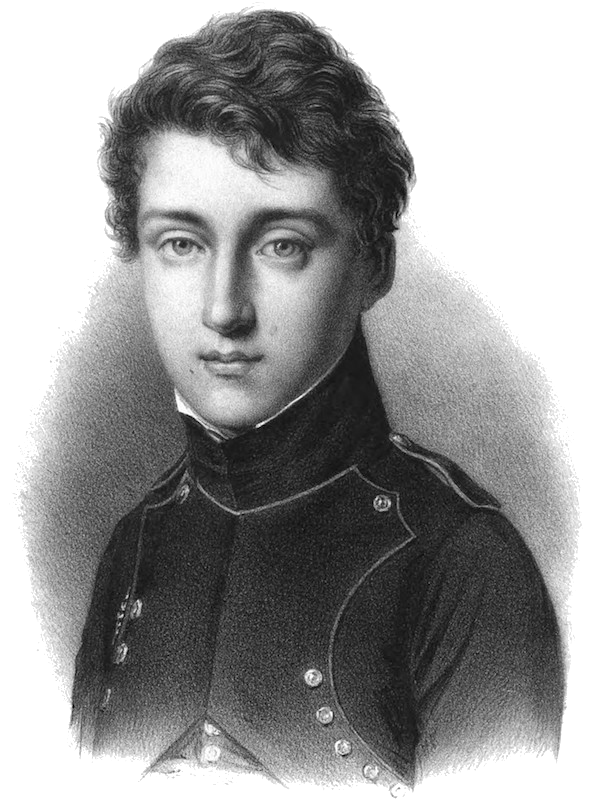
\includegraphics[scale=.15]{Nicolas-Leonard-Sadi-Carnot}\\
			\text{\DS លោក សាឌីកាណូ}\\
			\text{ជនជាតិបារាំង(១៧៩៦-១៨៣២)}
		\end{figure}
	\end{minipage}
\end{biography}
សុិចកាណូ ដំណើរការជាខួបរេវែសុីប{\en(Reversible)} មានបួនដំណាក់កាលដែលក្នុងនោះមាន២ជាលំនាំអុីសូទែម និង ២ទៀតជាលំនាំអាដ្យាបាទិច។\\
ដំណើការរបស់សុិចកាណូត្រូវបានតាងលើដ្យាក្រាម $\left(PV\right)$ ដូចរូបខាងក្រោមៈ\\
	\begin{minipage}[l]{.5\textwidth}
		\begin{itemize}
			\item $A\rightarrow B$ ពង្រីកតាមលំនាំអុីសូទែម
			\item $B\rightarrow C$ ពង្រីកតាមលំនាំអាដ្យាបាទិច
			\item $C\rightarrow D$ បណ្ណែនតាមលំនាំអុីសូទែម
			\item $D\rightarrow A$ បណ្ណែនតាមលំនាំអាដ្យាបាទិច
		\end{itemize}
	\end{minipage}
	\begin{minipage}[r]{.6\textwidth}
		\begin{figure}[H]
			\centering
			\begin{tikzpicture}[
				> = latex,
				dot/.style = {draw,fill,circle,inner sep=1pt},
				arrow inside/.style = {postaction=decorate,decoration={markings,mark=at position .55 with \arrow{>}}}
				]
				\begin{scope}
				\draw[<->] (0,4.5) node[left] {$P$} |- (4.5,0) node[right] {$V$};
				\node[dot,label={above:$A$}] (@a) at (0.5,4) {};
				\node[dot,label={right:$B$}] (@b) at (2.5,3) {};
				\node[dot,label={right:$C$}] (@c) at (4,1) {};
				\node[dot,label={left:$D$}] (@d) at (1.5,2) {};
				\draw[arrow inside] (@a) to[looseness=.7,bend right=20] (@b);
				\draw[arrow inside] (@b) to[looseness=.7,bend right=20] (@c);
				\draw[arrow inside] (@c) to[looseness=.7,bend left=20] (@d);
				\draw[arrow inside] (@d) to[looseness=.7,bend left=20] (@a);
				\draw[->, line width=3pt] (2,3.5) -- (2,2.5);
				\draw[->, line width=3pt] (2,2) -- (2,1);
				\node[label={above:$Q_{h}$}] at (2,3.5) {};
				\node[label={below:$Q_{c}$}] at (2,1) {};
				\draw[dashed] (@a)--(.5,0);
				\draw[dashed] (@b)--(2.5,0);
				\draw[dashed] (@c)--(4,0);
				\draw[dashed] (@d)--(1.5,0);
				\coordinate[label=below:$V_{A}$] (VA) at (.5,0);
				\coordinate[label=below:$V_{B}$] (VB) at (2.5,0);
				\coordinate[label=below:$V_{C}$] (VC) at (4,0);
				\coordinate[label=below:$V_{D}$] (VD) at (1.5,0);
				\end{scope}
			\end{tikzpicture}
			\caption{ដ្យាក្រាមសុិចកាណូ}
		\end{figure}
	\end{minipage}
\begin{enumerate}
	\item \emph{\DS តាមគន្លងនីមួយៗយើងអាចបកស្រាយដូចខាងក្រោម៖}
	\begin{itemize}
		\item [$-$] គន្លង $AB:$ ឧស្ម័នត្រូវបានរីកតាមលំនាំអុីសូទែម។ គេបាន $\Delta T=0$ នោះ $\Delta U=0$ ដែរ។\\
		តាមច្បាប់ទី១ ទែម៉ូឌីណាមិច $Q=W+\Delta U\Rightarrow W=Q$ មានន័យថា បរិមាណកម្តៅ $Q_{h}$ ដែលបានស្រូបដោយឧស្ម័ន ពីធុងក្តៅដែលមានសីតុណ្ហភាព $T_{h}$ ស្មើនឹងកម្មន្ត $W_{AB}$ ដែលធ្វើដោយឧស្ម័នក្នុងដំណើរការនេះ។
		\item [$-$] គន្លង $BC:$ ឧស្ម័នត្រូវបានរីកតាមលំនាំអាដ្យាបាទិច។ គេបាន $Q_{h}=Q_{c}$ នោះ $Q=0$។\\
		តាមច្បាប់ទី១ ទែម៉ូឌីណាមិច $Q=W+\Delta U\Rightarrow W=\Delta U$ មានន័យថា ថាមពលចាំបាច់សម្រាប់ធ្វើកម្មន្ត $W_{BC}$ ដែលធ្វើឡើងដោយឧស្ម័នក្នុងដំណើរការ $BC$ បានមកពីតំហយថាមពលក្នុងនៃឧស្ម័ននោះ នៅពេលដែលឧស្ម័នថយចុះពីសីតុណ្ហភាព $T_{h}$ ទៅ $T_{c}$។
		\item [$-$] គន្លង $CD:$ ឧស្ម័នបណ្ណែនតាមលំនាំអុីសូទែម។ គេបាន $\Delta T=0$ ហើយ $\Delta U=0$។ តាមច្បាប់ទី១ទែម៉ូឌីណាមិច $Q=W+\Delta U\Rightarrow Q=W$ មានន័យថាកម្មន្ត $W_{CD}$ ដែលធ្វើលើឧស្ម័នក្នុងគន្លង $AB$ នេះស្មើនឹងកម្តៅដែលដកចេញពីឧស្ម័ន $\left(Q_{c}\right)$ នៅសីតុណ្ហភាព $T_{c}$។
		\item [$-$] គន្លង $DA:$ ឧស្ម័នបណ្ណែនតាមលំនាំអាដ្យាបាទិច។ គេបាន $Q_{h}=Q_{c}$ នោះ $Q=0$។\\
		តាមច្បាប់ទី១ ទែម៉ូឌីណាមិច $Q=W+\Delta U\Rightarrow W=\Delta U$ មានន័យថា ថាមពលចាំបាច់សម្រាប់ធ្វើកម្មន្ត $W_{DA}$ ដែលធ្វើឡើងដោយឧស្ម័នក្នុងដំណើរការ $DA$ ស្មើនឹងការកើនឡើងនៃថាមពលក្នុងរបស់ឧស្ម័ន នៅពេលឧស្ម័នមានសីតុណ្ហភាពកើនឡើងពី $T_{c}$ ទៅ $T_{h}$។
	\end{itemize}
	\item \emph{\kml ទ្រឹស្តីបទកាណូ} បានពោលដូចតទៅៈ
	\begin{itemize}
		\item ម៉ាសុីន ឬម៉ូទ័រប្រើកម្តៅដែលមានប្រភពកម្តៅពីរ មានទិន្នផលកម្តៅអតិបរមាកាលណាការបញ្ចូនកម្តៅមានលំនាំរេវែសុីប{\en(Reversible Process)}។
		\item ទិន្នផលកម្តៅមិនអាស្រ័យនឹងប្រភេទប្រភពកម្តៅ ឬលំនាំនៃសិុចរេវែសុីប{\en(Process of Reversible Cycle)} ទេ។
		\item ទិន្នផលកម្តៅអតិបរមាអាស្រ័យតែនឹងសីតុណ្ហភាពដាច់ខាតនៃប្រភពកម្តៅ $T_{h}$ និងប្រភពត្រជាក់ $T_{c}$។
	\end{itemize}
	\begin{flalign*}
		\text{យើងបានទិន្នផលកម្តៅអតិបរមា}\quad :& \quad e_{C}=\frac{\Delta T}{T_{h}}=\frac{T_{h}-T_{c}}{T_{h}}=1-\frac{T_{c}}{T_{h}}\quad\text{\en Carnot(ideal) Efficiency}
	\end{flalign*}
\end{enumerate}
\subsection{ម៉ាសុីនអុីដេអាល់}
ចំពោះម៉ាសុីនអុីដេអាល់ យើងបានកម្តៅសមាមាត្រនឹងសីតុណ្ហភាពៈ $\frac{T_{h}}{T_{c}}=\frac{Q_{h}}{Q_{c}}$
\begin{flalign*}
	\text{គេអាចសរសេរ}\quad :&\quad e_{C}=1-\frac{Q_{c}}{Q_{h}}=\frac{Q_{h}-Q_{c}}{Q_{h}}=\frac{W}{Q_{h}}\\
	\text{ដូចនេះ}\quad :&\quad e_{C}=\frac{W}{Q_{h}}\left(\text{ជាទិន្នផលកម្តៅអតិបរមា}\right)
\end{flalign*}
\section{ម៉ាសុីនពិត(ម៉ាសុីនសាំង,ម៉ាសុីនម៉ាស៊ូត)}
\subsection{ម៉ាសុីនសាំងបន្ទុះបួនវគ្គ}
ម៉ូទ័រទាំងឡាយណាដែលធ្វើឲ្យកម្តៅក្លាយជាកម្មន្ត ហៅថា ម៉ូទ័រកម្តៅ ឬម៉ាសុីនកម្តៅ។ គេបានបែងចែកម៉ូទ័រចំហេះជាពីរគឺម៉ូទ័រចំហេះក្នុង និងម៉ូទ័រចំហេះក្រៅ។
\begin{itemize}
	\item \emph{\kml ម៉ូទ័រចំហេះក្រៅៈ} ជាប្រភេទម៉ូទ័រដែលបន្ទប់ចំហេះស្ថិតនៅក្រៅកន្លែង ដែលកម្តៅត្រូវបានធ្វើទៅជា កម្មន្ត។\\
	ឧទាហរណ៍ៈ ម៉ាសុីនប្រើចំហាយទឹក ទួប៊ីនប្រើចំហាយទឹក។ ល។(ខ្ញុំបានបង្ហាញនៅចំណុចខាងលើរួចហើយនៃគំរូម៉ាសុីនចំហាយទឹក)
	\item \emph{\kml ម៉ូទ័រចំហេះក្នុងៈ} ជាប្រភេទម៉ូទ័រដែលបន្ទប់ចំហេះស្ថិតនៅក្នុងកន្លែង ដែលកម្តៅត្រូវបានធ្វើទៅជា កម្មន្ត។\\
	ឧទាហរណ៍ៈ ម៉ាសុីនសាំង ម៉ាសុីនម៉ាស៊ូត។\\
	ម៉ូទ័រចំហេះក្នុងចែកចេញជាពីរប្រភេទទៅតាមបច្ចេកទេសនៃការឆេះរបស់ល្បាយ ប្រេងឥន្ទនៈ ខ្យល់ គឺ៖
	\begin{itemize}
		\item ម៉ូទ័រដែលបញ្ឆេះដោយបញ្ជា(ម៉ូទ័រសាំង)
		\item ម៉ូទ័រដែលបញ្ឆេះដោយបណ្ណែន(ម៉ូទ័រម៉ាស៊ូត)
	\end{itemize}
	\begin{enumerate}
		\item \emph{\kml ម៉ូទ័របន្ទុះបួនវគ្គ} ដំណើរការមានដូចតទៅៈ
		\begin{itemize}
			\item វគ្គទី១(ស្រូប ឬសម្រូប): ពិស្តុងធ្លាក់ចុះក្រោម ស៊ូបាប់ស្រូបបើកលាយល្យាយចំហាយសាំង-ខ្យល់។
			\item វគ្គទី២(បណ្ណែន): ស៊ូបាប់ស្រូបបិទ ពិស្តុងផ្លាស់ទីឡើងលើបណ្ណែនល្បាយចំហាយសាំង-ខ្យល់។
			\item វគ្គទី៣(បន្ទុះ និងបន្ធូ): ប៊ូសុីបញ្ចេញផ្កាភ្លើង ធ្វើឲ្យឆេះល្បាយសាំង-ខ្យល់។\\ ឧស្ម័នរីកមាឌធាក់ពិស្តុងចុះក្រោមវិញ(វគ្គនេះជាវគ្គដែលបង្កើតកម្មន្ត)
			\item វគ្គទី៤(បញ្ចេញ): ពិស្តុងផ្លាស់ទីឡើងលើ ស៊ូប៉ាប់បញ្ចេញបើកបញ្ចេញចំហេះឧស្ម័នទៅក្រៅ។
		\end{itemize}
		\begin{figure}[H]
			\centering
			\begin{subfigure}{.2\textwidth}
				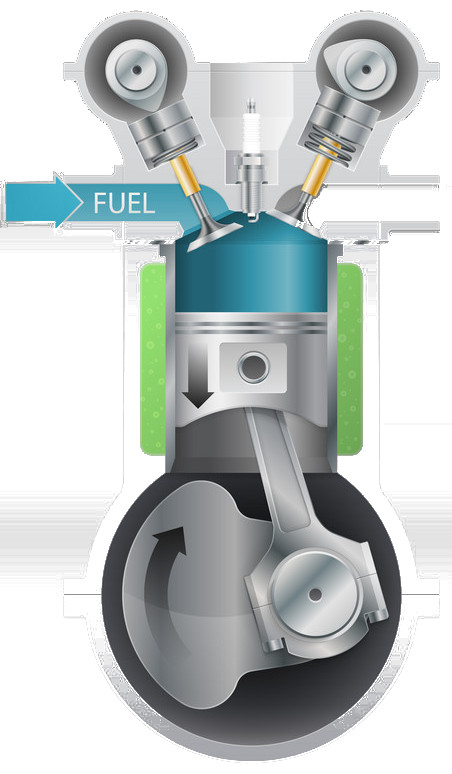
\includegraphics[scale=.2]{first-stroke}
				\subcaption{\DS វគ្គសម្រូប}
			\end{subfigure}
			\begin{subfigure}{.2\textwidth}
				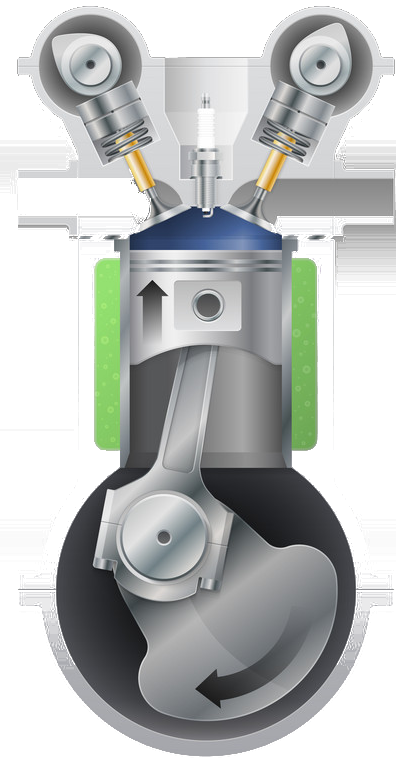
\includegraphics[scale=.2]{second-stroke}
				\subcaption{\DS វគ្គបណ្ណែន}
			\end{subfigure}
			\begin{subfigure}{.2\textwidth}
				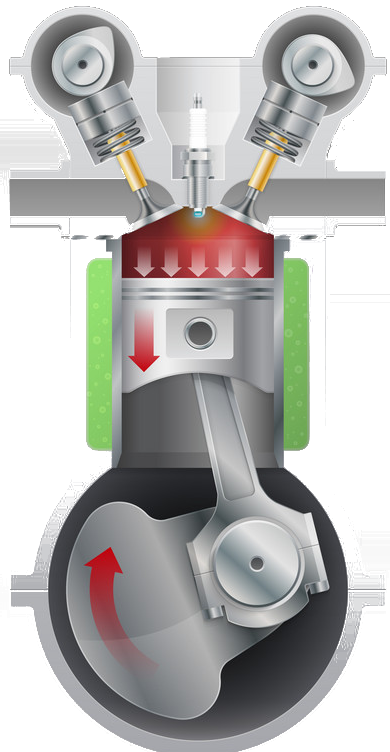
\includegraphics[scale=.2]{thirth-stroke}
				\subcaption{\DS វគ្គបន្ទុះ និងបន្ធូ}
			\end{subfigure}
			\begin{subfigure}{.2\textwidth}
				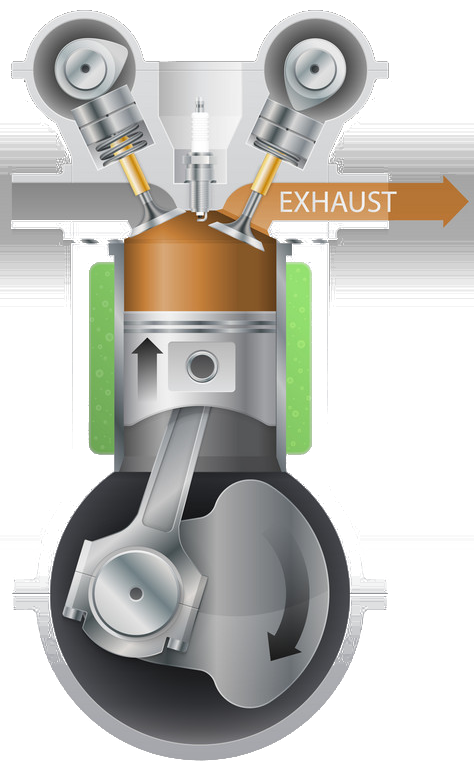
\includegraphics[scale=.2]{fourth-stroke}
				\subcaption{\DS វគ្គបញ្ចេញ}
			\end{subfigure}
			\caption{ដំណើរការម៉ូទ័របន្ទុះបួនវគ្គ}
		\end{figure}
		\item \emph{\kml ម៉ូទ័រសាំងលាយបន្ទុះពីរវគ្គ} ដំណើរការមានដូចតទៅៈ
		\begin{itemize}
			\item វគ្គទី១(បណ្ណែន និងបន្ទុះ): ពិស្តុងផ្លាស់ទីឡើងលើបិទរន្ធបញ្ចេញ ល្យាយចំហាយសាំង-ខ្យល់មួយភាគត្រូវបានបណ្ណែន។ មុនពេលពិស្តុងឡើងដល់ ចំណុចខ្ពស់បំផុត ប៊ូសុីបាញ់ភ្លើងធ្វើឧស្ម័នរីកមាឌផ្ទុះឡើង។
			\item វគ្គទី២(ស្រូប និងបញ្ចេញ): ពិស្តុងធ្លាក់យ៉ាងរហ័សបន្ទាប់ពីផ្ទុះ។ តួពីស្តុងក៏បិទរន្ធស្រូបវិញ និងបើករន្ធបញ្ចេញពេលធ្លាកដល់ក្រោមបំផុតដែលធ្វើឲ្យឧស្ម័នអាចចេញក្រៅបាន។
		\end{itemize}
		\item \emph{\kml ម៉ូទ័រម៉ាស៊ូតបន្ទុះបួនវគ្គ} ដំណើរការមានដូចតទៅៈ 
		\begin{itemize}
			\item វគ្គទី១(សម្រូប): ស៊ូប៉ាប់ស្រូបបើក ពិស្តុងផ្លាស់ទីទទួលខ្យល់ធ្វើឲ្យមានកំណើនមាឌតាមលំនាំអុីសូបារ។
			\item វគ្គទី២(បណ្ណែន): ស៊ូប៉ាប់ទាំងពីរបិទជិត ពិស្តុងផ្លាស់ទីបណ្ណែនខ្យល់ធ្វើឲ្យសម្ពាធខ្យល់កើនឡើងតាមលំនាំអុីសូទែម។
			\item វគ្គទី៣(បន្ទុះ និងបន្ធូ): ពិស្តុងផ្លាស់ទីដល់ចំណុចដើមតាមលំនាំអុីសូបារ សីតុណ្ហភាពកើនឡើងខ្លាំង។ ប្រេងម៉ាស៊ូតក៏ត្រូវបានបាញចូល និងឆេះដោយខ្យល់ក្តៅ។ ឧស្ម័នរីកមាឌតាមលំនាំអុីសូទែម រុញពិស្តុងចេញវិញ។
			\item វគ្គទី៤(បញ្ចេញ): ពិស្តុងផ្លាស់ទីបង្រួមមាឌឧស្ម័ន ស៊ូប៉ាប់បញ្ចេញបើក ឯប៉ាប់ស្រូបបិទធ្វើឧ្យម៉ាស៊ូតដែលឆេះស្ទុះចេញក្រៅរហូតឆេះអស់។
		\end{itemize}
		\item \emph{\kml ទិន្នផលនៃម៉ាសុីនកម្តៅ}
			\begin{itemize}
				\item [$\bullet$] \emph{\kml ដ្យាក្រាមតុល្យភាពថាមពល}
				\begin{figure}[H]
					\centering
					\begin{tikzpicture}
					\begin{scope}
					\filldraw[orange, fill=yellow!60!white] (0,0) circle (1.5cm);
					\filldraw[blue, fill=blue!20!white] (6,0) circle (1.5cm);
					\draw[->, >=latex, red!80!black, line width=10pt] (-5,0) to (-1.5,0);
					\draw[->, >=latex, green!60!black, line width=10pt] (1.5,0) to (4.5,0);
					\draw[->, >=latex, green!60!black, line width=10pt] (7.5,0) to (10.5,0);
					\draw[->, >=latex, blue!60!black, line width=10pt] (0,-1.5) to (0,-4);
					\draw[->, >=latex, blue!60!black, line width=10pt] (6,-1.5) to (6,-4);
					\node at (0,0) {\textcolor{blue}{\DS បន្ទប់ចំហេះ}};
					\node at (6,0) {\textcolor{blue}{\DS ភ្លៅម៉ូទ័រ}};
					\node at (-3,1) {\text{\DS ស្រូបកម្តៅ $Q_{h}$}};
					\node at (3,1) {\text{\DS ផ្តល់កម្មន្ត $W_{M}$}};
					\node at (9,1) {\text{\DS ផ្តល់កម្មន្ត $W_{U}$}};
					\node at (-1,-4.3) {\text{\DS កម្តៅភាយចេញ $Q_{c}$}};
					\node at (5,-4.3) {\text{\DS កម្តៅភាយចេញ $Q'_{c}$}};
					\end{scope}
					\end{tikzpicture}
				\end{figure}
			ម៉ាសុីនប្រើកម្តៅចែកចេញជាពីរផ្នែកគឺ
			\item [$\bullet$] \emph{\kml ផ្នែកកម្តៅ(ផ្នែកបម្លែងកម្តៅៈ)} ម៉ាសុីនទទួលកម្តៅ $Q_{h}$ រួចបម្លែងទៅជាកម្មន្តមេកានិច $W_{M}$ និងបញ្ចេញកម្តៅ $Q_{c}$ ទៅក្នុងបរិយាកាស។
				\begin{enumerate}[k]
					\item \emph{\kml តុល្យភាពថាមពល៖} $Q_{h}=W_{M}+Q_{c}$ នោះ $W_{M}=Q_{h}-Q_{c}$
					\begin{flalign*}
						\text{ដែល៖}\quad &\quad Q_{h}\quad \text{កម្តៅស្រូបដោយម៉ាសុីន(ថាមពលសរុប)$\left(J\right)$}\\
						\quad &\quad W_{M}\quad\text{កម្មន្តមេកានិច$\left(J\right)$}\\
						\quad &\quad Q_{c}\quad \text{កម្តៅភាយចេញពីម៉ាសុីន(ថាមពលខាតបង់)$\left(J\right)$}
					\end{flalign*}
					\item \emph{\kml ទិន្នផលកម្តៅនៃម៉ាសុីន៖} $e_{C}=\frac{W_{M}}{Q_{h}}=1-\frac{Q_{c}}{Q_{h}}$(ក្នុងបន្ទប់ចំហេះ)
				\end{enumerate}
			\item [$\bullet$] \emph{\kml ផ្នែកមេកានិច(ផ្នែកបញ្ចូនៈ)} កម្មន្តមេកានិច $W_{M}$ ត្រូវបានបញ្ចូនទៅជាកម្មន្តបានការ $W_{U}$ និងកម្តៅចេញពីម៉ាសុីនដោយកកិត $Q'_{c}$។
			\begin{enumerate}[k]
				\item \emph{\kml តុល្យភាពថាមពល៖} $W_{M}=W_{U}+Q'_{c}$
				\begin{flalign*}
				\quad &\quad W_{M}\quad\text{កម្មន្តមេកានិច$\left(J\right)$}\\
				\quad &\quad W_{U}\quad \text{កម្មន្តបានការ$\left(J\right)$}\\
				\quad &\quad Q'_{c}\quad \text{កម្តៅភាយចេញពីម៉ាសុីនដោយកកិត(ថាមពលខាតបង់)$\left(J\right)$}
				\end{flalign*}
				\item \emph{\kml ទិន្នផលមេកានិច ឬទិន្នផលនៃគ្រឿងបញ្ជូននៃម៉ាសុីនកម្តៅ៖} $e_{M}=\frac{W_{U}}{W_{M}}$(លើភ្លៅម៉ូទ័រ)
				\item \emph{\kml ទិន្នផលបានការ ឬទិន្នផលសរុប(ទិន្នផលពិត)}\\
				យើងបានទិន្នផលសរុប ឬទិន្នផលបានការនៃម៉ាសុីនគឺៈ
				\begin{flalign*}
				\quad &\quad e_{U}=\frac{W_{U}}{Q_{h}}\\
				\text{ដោយ}\quad :&\quad e_{M}=\frac{W_{U}}{W_{M}}\quad \text{នោះ}\quad W_{U}=e_{M}\times W_{M}\\
				\text{យើងបាន}\quad:&\quad e_{U}=\frac{e_{M}\times W_{M}}{Q_{h}}=e_{M}\times e_{C}\\
				\text{ដូចនេះ}\quad :&\quad e_{U}=\frac{W_{U}}{Q_{h}}=e_{M}\times e_{C}
				\end{flalign*}
			\end{enumerate}
				\item [$\bullet$] \emph{\kml អានុភាពមេកានិចរបស់ម៉ាសុីនៈ} $P=\frac{W}{t}$ ឬ $P_{M}=\frac{W_{M}}{t}$
				\begin{flalign*}
					\text{ដែល}\quad :&\quad P\quad \text{គិតជា} \left(W\right)\\
					\text{និង}\quad :&\quad t\quad \text{គិតជា}\left(s\right)
				\end{flalign*}
			\end{itemize}
		\begin{remark}
			ម៉ាសុីនសាំងមានទិន្នផលប្រហែល $30\%$ រីឯទិន្នផលម៉ាសុីនម៉ាស៊ូតប្រហែល $39\%$។ ទិន្នផលនៃគ្រឿងបញ្ចូនមានតម្លែ $90\%$ និងទិន្នផលបានការមានតម្លៃប្រហែល​ $30\%$។ ទិន្នផលនេះមានតម្លៃទាប។ ក្នុងចំណុះសាំង $10$ លីត្រ មានតែ $3$ លីត្រទេដែលផ្តល់កម្មន្តបានការ។ 
		\end{remark}
	\end{enumerate}
\end{itemize}
\begin{example}
	\begin{enumerate}
		\item រាលវិនាទី ម៉ូទ័ររថយន្តមួយទទួលកម្តៅ $172kJ$ ពីប្រតិកម្មនៃចំហេះល្យាយឧស្ម័ន និងបញ្ចេញមកបរិយាកាសក្រៅ $135kJ$។
		\begin{enumerate}[1]
			\item \begin{enumerate}[k]
				\item រៀបរាប់វគ្គទាំងបួននៃសុិច
				\item គណនាកម្មន្តមេកានិច ក្នុងរយៈពេល $10$ នាទី
				\item គណនាទិន្នផលកម្តៅនៃម៉ូទ័រ
			\end{enumerate}
			\item ទិន្នផលគ្រឿនបញ្ចូន $92\%$។
			\begin{enumerate}[k]
				\item គណនាកម្មន្តបានការដែលភ្លៅម៉ូទ័របានទទួលរយៈពេល $10$ នាទី។
				\item គណនាទិន្នផលបានការនៃម៉ាសុីន។
			\end{enumerate}
		\end{enumerate}
		\item ម៉ូទ័រម៉ាស៊ូតមួយទទួលកម្តៅ $3.83MJ$។ វាមានទិន្នផលកម្តៅ $0.45$។
		\begin{enumerate}
			\item គណនាកម្មន្តមេកានិចដែលផ្តល់ដោយពីស្តុង
			\item តើកម្តៅដែលបញ្ចេញទៅក្នុងបរិយាកាសមានតម្លៃប៉ុន្មាន?
			\item ទិន្នផលគ្រឿងបញ្ចូនគឺ $0.85$។ គណនាកម្មន្តដែលទទួលដោយភ្លៅម៉ូទ័រ។
		\end{enumerate}
	\end{enumerate}
\end{example}
\begin{center}
	{\Large \kml\color{magenta} ចប់ដោយសង្ខេប!!!}
\end{center}